\chapter{Optional Material}


\section{Interpolation}
The least squares problem that we studied in the previous sections seeks to find a best
fitting function that is {\it closest} (in the 2-norm sense) to a set of data.  What if,
instead, we want to match the data points \underline{exactly} with a function. This is the realm of
interpolation.  Take note that there are many many forms of interpolation that are
tailored to specific problems.  In this brief section we cover only a few of the simplest
forms of interpolation involving only polynomial functions.
The problem that we'll focus on can be phrased as:\\  Given a set of $n+1$ data points $(x_0, y_0), (x_1, y_1), \ldots,
(x_n,y_n)$, find a polynomial of degree at most $n$ that exactly fits these points.
\subsection{Vandemonde Interpolation}
We have technically already seen Vandermonde interpolation.  In Section
\ref{sec:least_squares} we built a system of equations to solve the least squares problem.
In the least squares problem we had more data points than unknown parameters resulting in
an over-determined system (look back to Section \ref{sec:least_squares} to remind
yourself).  If, however, we choose a polynomial model that has the same number of unknown
parameters as data points then the resulting system if not over-determined.

For example, let's say that we have the data set 
\[ S = \{ (0,1) \, , \, (1,2) \, , \, (2,5) \, , \, (3,10) \} \]
and we want to fit a polynomial then we can use a cubic function (which has 4 parameters)
to match the data perfectly.  Indeed, if we choose $p(x) = \beta_0 + \beta_1 x + \beta_2
x^2 + \beta_3 x^3$ then the resulting system of equations is
\[ \begin{pmatrix}  1 & 0 & 0 & 0 \\
                    1 & 1 & 1 & 1 \\
                    1 & 2 & 4 & 8 \\
                    1 & 3 & 9 & 27 \end{pmatrix} \begin{pmatrix} \beta_0 \\ \beta_1 \\
                    \beta_2 \\ \beta_3 \end{pmatrix} = \begin{pmatrix} 1 \\ 2 \\ 5 \\ 10
            \end{pmatrix}. \]

Notice that the system of equations is square, and solving using any method discussed in
this chapter results in $\beta_0 = 1$, $\beta_1 = 0$, $\beta_2 = 1$, and $\beta_3 = 0$.
Hence, the interpolating function is $p(x) = 1 + 0x + 1x^2 + 0x^3 = 1+x^2$, and we know
that $p(x)$ matches this data set perfectly as seen in Figure \ref{fig:vandermonde}.

\begin{figure}[ht!]
    \begin{center}
        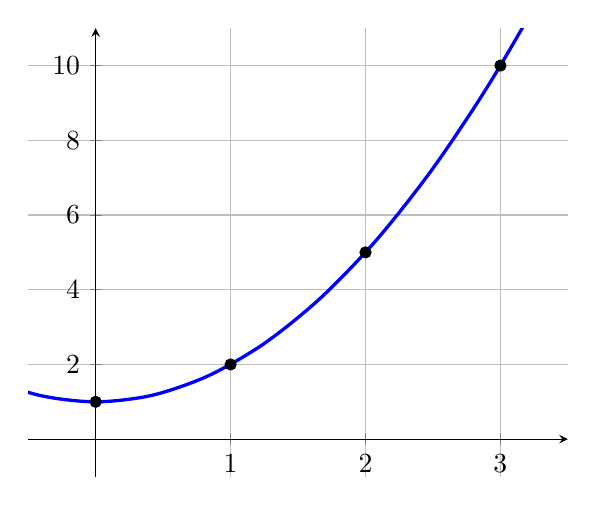
\begin{tikzpicture}
            \begin{axis}[axis lines=center, grid, xmin=-0.5, xmax=3.5, ymin=-1, ymax=11]
                \addplot[smooth, very thick, blue] {x^2 + 1};
                \addplot[mark=*, only marks] coordinates{(0,1)(1,2)(2,5)(3,10)};
            \end{axis}
        \end{tikzpicture}
    \end{center}
    \caption{A simple Vandermonde interpolation for the data set $S = \{(0,1) \, , \,
(1,2) \, , \, (2,5) \, , \, (3,10) \}$ resulting in the interpolating function $p(x) =
1+x^2$.}
    \label{fig:vandermonde}
\end{figure}


\begin{problem}\label{prob:vandermonde_1}
   Write a MATLAB function that accepts a list of ordered pairs (where each $x$ value is
   unique) and builds a Vandermonde interpolation polynomial.  Test your function on the
   simple example listed above and then on several larger problems.  It may be simplest to
   initially test on functions that we know.
\end{problem}

\begin{problem}
    Build a Vandermonde interpolation polynomial to interpolate the function $f(x) =
    \cos(2 \pi x)$ with 10 points that are linearly spaced on the interval $x \in [0,2]$.
\end{problem}

\begin{definition}[The Vandermonde Matrix]
    Let $S = \{(x_0,y_0) \,,\, (x_1,y_1) \,,\, \ldots, (x_n,y_n)\}$ be a list of ordered
    pairs where the $x$ values are all unique.  Using Vandermonde interpolation we arrive
    at the system of equations
    \begin{flalign}
        \begin{pmatrix} 1 & x_0 & x_0^2 & \cdots & x_0^n \\
                        1 & x_1 & x_1^2 & \cdots & x_1^n \\
                        1 & x_2 & x_2^2 & \cdots & x_2^n \\
                        \vdots & \vdots & \vdots & \ddots & \vdots \\
                        1 & x_n & x_n^2 & \cdots & x_n^n \end{pmatrix}
        \begin{pmatrix} \beta_0 \\ \beta_1 \\ \beta_2 \\ \vdots \\ \beta_n \end{pmatrix}
        =
        \begin{pmatrix} y_0 \\ y_1 \\ y_2 \\ \vdots \\ y_n \end{pmatrix}.
        \label{eqn:vandermonde}
    \end{flalign}
    The matrix on the left-hand side of \eqref{eqn:vandermonde} is called the {\bf
    Vandermonde Matrix}.
\end{definition}

\begin{problem}
    Vandermonde matrix is relatively easy to conceptualize and code, but there is an
    inherent problem.  Use your code from Problem \ref{prob:vandermonde_1} to create a
    plot on a \mcode{semilogy} scale.  The horizontal axis of the plot is the order of the
    interpolating polynomial and the vertical axis is the ratio
    $|\lambda_{max}|/|\lambda_{min}|$ where $\lambda_{max}$ and $\lambda_{min}$ are the
    maximum and minimum eigenvalues of the Vandermonde matrix respectively.  What does
    this plot tell you about Vandermonde interpolation for high-order polynomials?
\end{problem}

\subsection{Lagrange Interpolation}
Lagrange interpolation is a rather clever interpolation scheme where we build up the
polynomial from simpler polynomials.  For interpolation we want to build a polynomial
$p(x)$ such that $p(x_j) = y_j$.  If we can find a polynomial $\phi_j(x)$ that 
\[ \phi_j(x) = \left\{ \begin{array}{ll} 0, & \text{ if } x = x_i \text{ and } i \ne j \\ 1, & \text{ if
    } x=x_j \end{array} \right. \]
then for Lagrange interpolation we build $p(x)$ as a linear combination of the $\phi_j$ functions.

\begin{problem}
    Consider the data set $S = \{(0,1) \, , \, (1,2) \, , \, (2,5) \, , \, (3,10) \}$.
    
    \begin{enumerate}
        \item[(a)] Based on the descriptions of the $p(x)$ and $\phi_j(x)$ functions, why would
            $p(x)$ be defined as
            \[ p(x) = 1 \phi_0(x) + 2 \phi_1(x) + 5 \phi_2(x) + 10 \phi_3(x)? \]
        \item[(b)] Verify that $\phi_0(x)$ can be defined as
            \[ \phi_0(x) = \frac{(x-1)(x-2)(x-3)}{(0-1)(0-2)(0-3)}. \]
        \item[(c)] Verify that $\phi_1(x)$ can be defined as
            \[ \phi_1(x) = \frac{(x-0)(x-2)(x-3)}{(1-0)(1-2)(1-3)}. \]
        \item[(d)] Define $\phi_2(x)$ and $\phi_3(x)$ in a similar way.
        \item[(e)] Build the linear combination from part (a) and create a plot showing that
            this polynomial indeed interpolates the points in the set $S$.
    \end{enumerate}
\end{problem}

\begin{technique}[Lagrange Interpolation]
    To build an interpolating polynomial $p(x)$ for the set of points
    $\{(x_0,y_0)\,,\,(x_1,y_1)\,,\,(x_2,y_2)\,,\ldots,\,(x_n,y_n)\}$ we first build the
    polynomials $\phi_j(x)$ for each $j = 0, 1, 2, \ldots, n$ and then construct the
    polynomial $p(x)$ as 
    \[ p(x) = \sum_{j=0}^n y_j \phi_j(x). \]
    The $\phi_j(x)$ functions are defined as
    \[ \phi_j(x) = \prod_{i \ne j} \frac{x-x_i}{x_j-x_i}. \]
\end{technique}

\begin{example}
    Build a Lagrange interpolation polynomial for the set of points
    \[ S  = \{(1,5)\,,\,(2,9)\,,\,(3,11)\}. \]
    {\bf Solution} \\
    We first build the three $\phi_j$ functions.
    \begin{flalign*}
        \phi_0(x) = \frac{(x-2)(x-3)}{(1-2)(1-3)} \\
        \phi_1(x) = \frac{(x-1)(x-3)}{(2-1)(2-3)} \\
        \phi_2(x) = \frac{(x-1)(x-2)}{(3-1)(3-2)}.
    \end{flalign*}
    Take careful note that the $\phi$ functions are built in a very particular way.
    Indeed, $\phi_0(1) = 1$, $\phi_0(2) =0$, and $\phi_0(3) = 0$.  Also, $\phi_1(1) = 0$,
    $\phi_1(2) = 1)$, and $\phi_1(3) = 0$.  Finally, note that $\phi_2(1) = 0$, $\phi_2(1)
    = 0$ and $\phi_2(3) = 1$.  Thus, the polynomial $p(x)$ can be built as
    \[ p(x) = 5 \phi_0(x) + 9 \phi_1(x) + 11 \phi(2(x) = 5 \frac{(x-2)(x-3)}{(1-2)(1-3)} +
    \frac{(x-1)(x-3)}{(2-1)(2-3)} + \frac{(x-1)(x-2)}{(3-1)(3-2)}. \]
    The remainder of the simplification is left to the reader.
\end{example}

\begin{problem}
    Write a MATLAB function that accepts a list of list of ordered pairs (where each $x$
    value is unique) and builds a Lagrange interpolation polynomial.  Test your function
    on the examples that we've presented in this section.
\end{problem}

\subsection{Interpolation at Chebyshev Points}
\begin{problem}
    Using either Vandermonde or Lagrange interpolation build a polynomial that
    interpolates the function 
    \[ f(x) = \frac{1}{1+x^2} \]
    for $x \in [-5,5]$
    with polynomials of order $n=2, 3, \ldots$ and linearly spaced interpolation
    points.  What do you notice about the
    quality of the interpolating polynomial near the endpoints?
    \begin{center}
        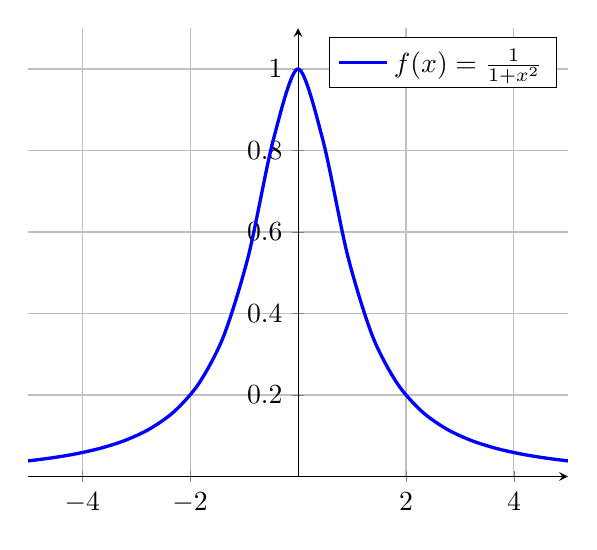
\begin{tikzpicture}
            \begin{axis}[axis lines=center, grid, domain=-5.5:5.5, xmin=-5, xmax=5,
                ymin=0, ymax=1.1] 
                \addplot[smooth, very thick, blue] {1/(1+x^2)};
                \addlegendentry{$f(x) = \frac{1}{1+x^2}$};
            \end{axis}
        \end{tikzpicture}
    \end{center}
\end{problem}

As you should have noticed the quality of the interpolation gets rather terrible near the
endpoints when you use linearly spaced points for the interpolation.  A fix to this was
first proposed by the Russian mathematician Pafnuty Chebyshev (1821-1894).  The idea is as
follows:
\begin{itemize}
    \item Draw a semicircle above the closed interval on which you are interpolating
        (shown in black in Figure \ref{fig:chebyshev_nodes}).
    \item Pick $n$ equally spaced points along the semicircle (i.e. same arc length between
        each point).  (shown in blue in Figure \ref{fig:chebyshev_nodes})
    \item Project the points on the semicircle down to the interval.  Use these projected
        points for the interpolation. (shown in red in Figure \ref{fig:chebyshev_nodes})
\end{itemize}

\begin{figure}
    \begin{center}
        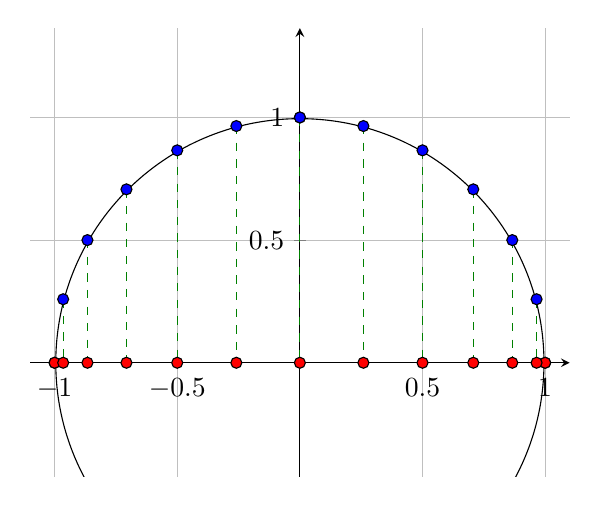
\begin{tikzpicture}
            \begin{axis}[axis equal, axis lines=center, xmin=-1.1, xmax=1.1, ymin=-0.2, ymax=1.1,
                grid]
%                 \addplot[smooth, very thick, samples=200] {sqrt(1-x^2)};
                %
                \draw[dashed, color=green!50!black] (axis cs:1,0) -- (axis cs:1,0);
                \draw[dashed, color=green!50!black] (axis cs:0.965,0.259) -- (axis cs:0.965,0);
                \draw[dashed, color=green!50!black] (axis cs:0.866,0.5) -- (axis cs:0.866,0);
                \draw[dashed, color=green!50!black] (axis cs:0.707,0.707) -- (axis cs:0.707,0);
                \draw[dashed, color=green!50!black] (axis cs:0.5,0.866) -- (axis cs:0.5,0);
                \draw[dashed, color=green!50!black] (axis cs:0.259,0.965) -- (axis cs:0.259,0);
                \draw[dashed, color=green!50!black] (axis cs:0,1) -- (axis cs:0,0);
                \draw[dashed, color=green!50!black] (axis cs:-1,0) -- (axis cs:-1,0);
                \draw[dashed, color=green!50!black] (axis cs:-0.965,0.259) -- (axis cs:-0.965,0);
                \draw[dashed, color=green!50!black] (axis cs:-0.866,0.5) -- (axis cs:-0.866,0);
                \draw[dashed, color=green!50!black] (axis cs:-0.707,0.707) -- (axis cs:-0.707,0);
                \draw[dashed, color=green!50!black] (axis cs:-0.5,0.866) -- (axis cs:-0.5,0);
                \draw[dashed, color=green!50!black] (axis cs:-0.259,0.965) -- (axis cs:-0.259,0);
                \draw[dashed, color=green!50!black] (axis cs:-0,1) -- (axis cs:-0,0);
                %
                \draw[black] (axis cs:0,0) circle(3.1cm);
                \draw[fill=blue] (axis cs:1,0) circle(0.07cm);
                \draw[fill=blue] (axis cs:0.965,0.259) circle(0.07cm);
                \draw[fill=blue] (axis cs:0.866,0.5) circle(0.07cm);
                \draw[fill=blue] (axis cs:0.707,0.707) circle(0.07cm);
                \draw[fill=blue] (axis cs:0.5,0.866) circle(0.07cm);
                \draw[fill=blue] (axis cs:0.259,0.965) circle(0.07cm);
                \draw[fill=blue] (axis cs:0,1) circle(0.07cm);
                \draw[fill=blue] (axis cs:-1,0) circle(0.07cm);
                \draw[fill=blue] (axis cs:-0.965,0.259) circle(0.07cm);
                \draw[fill=blue] (axis cs:-0.866,0.5) circle(0.07cm);
                \draw[fill=blue] (axis cs:-0.707,0.707) circle(0.07cm);
                \draw[fill=blue] (axis cs:-0.5,0.866) circle(0.07cm);
                \draw[fill=blue] (axis cs:-0.259,0.965) circle(0.07cm);
                \draw[fill=blue] (axis cs:-0,1) circle(0.07cm);
                %
                \draw[fill=red] (axis cs:1,0) circle(0.07cm);
                \draw[fill=red] (axis cs:0.965,0) circle(0.07cm);
                \draw[fill=red] (axis cs:0.866,0) circle(0.07cm);
                \draw[fill=red] (axis cs:0.707,0) circle(0.07cm);
                \draw[fill=red] (axis cs:0.5,0) circle(0.07cm);
                \draw[fill=red] (axis cs:0.259,0) circle(0.07cm);
                \draw[fill=red] (axis cs:0,0) circle(0.07cm);
                \draw[fill=red] (axis cs:-1,0) circle(0.07cm);
                \draw[fill=red] (axis cs:-0.965,0) circle(0.07cm);
                \draw[fill=red] (axis cs:-0.866,0) circle(0.07cm);
                \draw[fill=red] (axis cs:-0.707,0) circle(0.07cm);
                \draw[fill=red] (axis cs:-0.5,0) circle(0.07cm);
                \draw[fill=red] (axis cs:-0.259,0) circle(0.07cm);
            \end{axis}
        \end{tikzpicture}
    \end{center}
    \caption{Chebyshev interpolation nodes for the interval $[-1,1]$. In this case each
    node is separated by $\pi/8$ radians giving 13 interpolations points including the
endpoints.}
    \label{fig:chebyshev_nodes}
\end{figure}

It should be clear that since we are projecting down to the $x$-axis from a circle then
all we need are the cosine values from the circle.  Hence we can form the Chebyshev
interpolation points from the formula
\begin{flalign}
    x_j = \cos\left( \frac{\pi j}{n} \right), \quad \text{for} \quad j=0, 1, \ldots, n
    \label{eqn:chebyshev_cosine}
\end{flalign}
on the interval $[-1,1]$.  

To transform the Chebyshev points from the interval $[-1,1]$ (found with
\eqref{eqn:chebyshev_cosine}) to the interval $[a,b]$ we can apply a linear function which
maps $-1$ to $a$ and $1$ to $b$:
\[ x_j \gets \left( \frac{b-a}{2} \right)\left( x_j + 1 \right) + a \]
where the ``$x_j$'' on the left is on the interval $[a,b]$ and the ``$x_j$'' on the right
is on the interval $[-1,1]$.

\begin{problem}
    Consider the function $f(x) = \frac{1}{1+x^2}$ just as we did for the first problem in
    this subsection.  Write MATLAB code that overlays an interpolation with linearly spaced
    points an interpolation with Chebyshev nodes.  Give plots for polynomial of order
    $n=2,3, 4, \ldots$.  Be sure to show the original function on your plots as well.
\end{problem}

\begin{problem}
    Demonstrate that the Chebyshev interpolation nodes will improve the stability of the
    Vandermonde matrix over using linearly spaced nodes.
\end{problem}

% \subsection{Cubic Splines}

\newpage\section{Low Rank Approximations of Matrices}

\begin{problem}
    One particular use of the SVD is for data reduction.  The word ``reduction'' here
    really means that we are going to make approximations of data using lower dimensions,
    and a very visually stunning way to do this is to do data reduction on images.  The following code will read
    the file \mcode{TestImage.jpg} into MATLAB and convert it to a rectangular matrix of
    values.  It is up to the reader to supply the necessary image.
\begin{lstlisting}
A = imread('TestImage.jpg');
A = A(:,:,1);
A = im2double(A);
imshow(A)
\end{lstlisting}
    Once the matrix is in MATLAB do the following.  In this we assume that $A$ is an $m
    \times n$ matrix.
    \begin{enumerate}
        \item Find the SVD of the image (remember the semicolons!!!!!!).  This will take
            over a minute with our code so be patient.  Once it is done check that your
            SVD code does a decent approximation of the original image.
\begin{lstlisting}
[U,S,V] = MySVD(A);
error = norm(A - U*S*V')
\end{lstlisting}
        \item Get the singular values out of $\Sigma$ and find the largest $P$\% of the
            singular values. Let's say that this is $N$ values.  Create four new matrices
            $U_{new}$, $\Sigma_{new}$, $V_{new}$, and $A_{new}$ in the following way.
            \begin{enumerate}
                \item $U_{new}$ is $m \times N$ and contains only the first $N$ columns of
                    $U$.
                \item $\Sigma_{new}$ is $N \times N$ and contains only the top $P$\% of
                    the singular values of $A$.
                \item $V_{new}$ is $n \times N$ and contains the first $N$ columns of $V$.
                \item $A_{new}$ is $m \times n$ and is formed by $U_{new} \Sigma_{new}
                    V_{new}^T$.  
            \end{enumerate}
        \item Show the newly data-reduced image with \\
            \mcode{imshow(Anew)}
        \item The rank of the new image is equal to the number of singular values that you
            kept in step 2.  
        \item Experiment with several low rank approximations of an image starting with
            rank 1 and progress up to larger and larger ranks matrices.  You'll find that
            the rank necessary to recover the full image is much lower than than the full
            original rank.
    \end{enumerate}
\end{problem}


\newpage\section{The Google Page Rank Algorithm}
In this section you will discover how the PageRank algorithm works to give the most relevant
information as the top hit on a Google search.  

Search engines compile large indexes of the dynamic information on the Internet so they
are easily searched.  This means that when you do a Google search, you are not actually
searching the Internet; instead, you are searching the indexes at Google.

When you type a query into Google the following two steps take place:
\begin{enumerate}
    \item Query Module: The query module at Google converts your natural language into a
        language that the search system can understand and consults the various indexes
        at Google in order to answer the query.  This is done to find the list of relevant
        pages.
    \item Ranking Module: The ranking module takes the set of relevant pages and ranks
        them. The outcome of the ranking is an ordered list of web pages such
        that the pages near the top of the list are most likely to be what you desire from
        your search. This ranking is the same as assigning a {\it popularity score} to
        each web site and then listing the relevant sites by this score.  
\end{enumerate}

This section focuses on the Linear Algebra behind the Ranking Module developed by the
founders of Google: Sergey Brin and Larry Page.  Their algorithm is called the
\emph{PageRank algorithm}, and you use it every single time you use Google's search
engine.


In simple terms: {\it A webpage is important if it is pointed to by other important
pages}.

The Internet can be viewed as a directed graph (look up this term
\href{https://en.wikipedia.org/wiki/Directed_graph}{here on Wikipedia}) where the nodes
are the web pages and the edges are the hyperlinks between the pages. The hyperlinks into a
page are called {\it inlinks}, and the ones pointing out of a page are called {\it
outlinks}.  In essence, a hyperlink from my page to yours is my endorsement of your page.
Thus, a page with more recommendations must be more important than a page with a few
links.  However, the status of the recommendation is also important. 

Let us now translate this into mathematics. To help understand
this we first consider the small web of six pages shown in Figure
\ref{fig:example_graph} (a graph of the router level of the internet can be found
\href{https://personalpages.manchester.ac.uk/staff/m.dodge/cybergeography/atlas/lumeta_large.jpg}{here}).  The links between the
pages are shown by arrows. An arrow pointing into a node is an {\it inlink}
and an arrow pointing out of a node is an {\it outlink}. In Figure
\ref{fig:example_graph}, node 3 has three outlinks (to nodes 1, 2, and 5)
and 1 inlink (from node 1).

\begin{figure}[ht]
    \begin{center}
        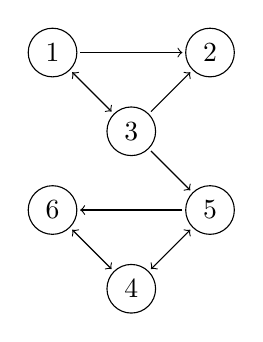
\begin{tikzpicture}
            \draw (0,0) node[circle,draw]{3};
            \draw (-1,1) node[circle,draw]{1};
            \draw (1,1) node[circle,draw]{2};
            \draw (-1,-1) node[circle,draw]{6};
            \draw (1,-1) node[circle,draw]{5};
            \draw (0,-2) node[circle,draw]{4};
        %
            \draw[<->] (-0.25,0.25) -- (-0.75,0.75);
            \draw[->] (-0.65,1) -- (0.65,1);
            \draw[->] (0.25,0.25) -- (0.75,0.75);
            \draw[->] (0.25,-0.25) -- (0.75,-0.75);
            \draw[->] (0.65,-1) -- (-0.65,-1);
            \draw[<->] (-0.75,-1.25) -- (-.25,-1.75);
            \draw[<->] (0.75,-1.25) -- (0.25,-1.75);
        \end{tikzpicture}
    \end{center}
        \caption{Sample graph of a web with six pages.}
        \label{fig:example_graph}
\end{figure}

We will first define some notation in the PageRank algorithm:
\begin{itemize}
    \item $|P_i|$ is the number of outlinks from page $P_i$
    \item $H$ is the {\it hyperlink} matrix defined as 
        \[ H_{ij} = \left\{ \begin{array}{cl} \frac{1}{|P_j|}, & \text{if there is a link
            from node $j$ to node $i$} \\ 0, & \text{otherwise} \end{array} \right. \]
        where the ``$i$'' and ``$j$'' are the row and column indices respectively.  
    \item $\bx$ is a vector that contains all of the PageRanks for the individual pages.
\end{itemize}

The PageRank algorithm works as follows:
\begin{enumerate}
    \item Initialize the page ranks to all be equal. This means that our initial
        assumption is that all pages are of equal rank.  In the case of Figure
        \ref{fig:example_graph} we would take $\bx_0$ to be 
        \[ \bx_0 = \begin{pmatrix} 1/6 \\ 1/6 \\ 1/6 \\ 1/6 \\ 1/6 \\ 1/6 \end{pmatrix}. \]
    \item Build the hyperlink matrix.  \\ As an example we'll consider node 3 in Figure
        \ref{fig:example_graph}.  There are three outlinks from node 3 (to nodes 1, 2, and
        5).  Hence $H_{13}=1/3$, $H_{23} = 1/3$, and $H_{53} = 1/3$ and the partially
        complete hyperlink matrix is
        \[ H = \begin{pmatrix} 
                - & - & 1/3 & - & - & - \\
                - & - & 1/3 & - & - & - \\
                - & - & 0   & - & - & - \\
                - & - & 0   & - & - & - \\
                - & - & 1/3 & - & - & - \\
                - & - & 0   & - & - & - 
            \end{pmatrix} \]
    \item The difference equation $\bx_{n+1} = H \bx_n$ is used to iteratively refine the
        estimates of the page ranks.  You can view the iterations as a person visiting a
        page and then following a link at random, then following a random link on the next
        page, and the next, and the next, etc.  Hence we see
        that the iterations evolve exactly as expected for a difference equation.
        \begin{center}
            \begin{tabular}{|c|c|}
                \hline
                Iteration & New Page Rank Estimation \\ \hline \hline
                0 & $\bx_0$ \\
                1 & $\bx_1 = H \bx_0$ \\
                2 & $\bx_2 = H \bx_1 = H^2 \bx_0$ \\
                3 & $\bx_3 = H \bx_2 = H^3 \bx_0$ \\
                4 & $\bx_4 = H \bx_3 = H^4 \bx_0$ \\
                \vdots & \qquad \vdots \\
                $k$ & $\bx_k = H^k \bx_0$ \\ \hline
            \end{tabular}
        \end{center}
    \item When a steady state is reached we sort the resulting vector $\bx_k$ to give the
        page rank. The node (web page) with the highest rank will be the top search
        result, the second highest rank will be the second search result, and so on.
\end{enumerate}

It doesn't take much to see that this process can be very time consuming.  Think about
your typical web search with hundreds of thousands of hits; that makes a square matrix $H$
that has a size of hundreds of thousands of entries by hundreds of thousands of entries!
The matrix multiplications alone would take many minutes (or possibly many hours) for
every search! \dots but Brin and Page were pretty smart dudes!!


We now state a few theorems and definitions that will help us simplify the iterative
PageRank process.
\begin{thm}\label{thm:eigen_expand}
    If $A$ is an $n \times n$ matrix with $n$ linearly independent eigenvectors $\bv_1,
    \bv_2, \bv_3,$ $\ldots, \bv_n$ and associated eigenvalues $\lambda_1, \lambda_2,
    \lambda_3, \ldots, \lambda_n$ then for any initial vector $\bx \in \mathbb{R}^n$ we
    can write $A^k \bx$ as
    \[ A^k \bx = c_1 \lambda_1^k \bv_1 + c_2 \lambda_2^k \bv_2 + c_3 \lambda_3^k \bv_3 +
        \cdots c_n \lambda_n^k \bv_n \]
    where $c_1, c_2, c_3, \ldots, c_n$ are the constants found by expressing $\bx$ as a
    linear combination of the eigenvectors. \\Note: We can assume that the eigenvalues are ordered
    such that $\lambda_1 \ge \lambda_2 \ge \lambda_3 \ge \cdots \ge \lambda_n$.
\end{thm}
\begin{proof}
    (Prove the preceding theorem)
\end{proof}

\begin{definition}
    A {\bf probability vector} is a vector with entries on the interval $[0,1]$ that add up to 1. 
\end{definition}
\begin{definition}
    A {\bf stochastic matrix} is a square matrix whose columns are probability vectors.
\end{definition}

\begin{thm} \label{thm:largest_ev_stochastic}
    If $A$ is a stochastic $n \times n$ matrix then $A$ will have $n$ linearly independent
    eigenvectors.  Furthermore, the largest eigenvalue of a stochastic matrix will
    \underline{always} be $\lambda_1 = 1$ and the smallest eigenvalue  will always be
    nonnegative: $0 \le \lambda_n < 1$.
\end{thm}

Some of the following tasks will ask you to {\it prove} a statement or a theorem.  This
means to clearly write all of the logical and mathematical reasons why the statement is
true. Your proof should be absolutely crystal clear to anyone with a similar mathematical
background \dots if you are in doubt then have a peer from a different group read your
proof to you \underline{out loud}.

\begin{problem}
    Finish writing the hyperlink matrix $H$ from Figure \ref{fig:example_graph}.
\end{problem}

\begin{problem}
    Write MATLAB code to implement the iterative process defined previously. Make a plot
    that shows how the rank evolves over the iterations.
\end{problem}


\begin{problem}
    What must be true about a collection of $n$ pages such that an $n\times n$
        hyperlink matrix $H$ is a stochastic matrix.
\end{problem}

The statement of the next theorem is incomplete, but the proof is given to you.  Fill in
the blank in the statement of the theorem and provide a few sentences supporting your
answer.
\begin{thm}\label{thm:steady}
    If $A$ is an $n \times n$ stochastic matrix and $\bx_0$ is some initial vector
    for the difference equation $\bx_{n+1} = A \bx_n$, then the steady state
    vector is
    \[ \bx_{equilib} = \lim_{k \to\infty} A^k \bx_0 = \underline{\hspace{1in}}. \]
\end{thm}
\begin{proof}
    First note that $A$ is an $n \times n$ stochastic matrix so from Theorem
    \ref{thm:largest_ev_stochastic} we know that there are $n$ linearly
    independent eigenvectors.  We can then substitute
    the eigenvalues from Theorem \ref{thm:largest_ev_stochastic} in Theorem
    \ref{thm:eigen_expand}. Noting that if $0<\lambda_j<1$ we have $\lim_{k \to
    \infty} \lambda_j^k = 0$ the result follows immediately.
\end{proof}
\begin{problem}
    Discuss how Theorem \ref{thm:steady} greatly simplifies the PageRank iterative process
    described previously.  In other words: there is no reason to iterate at all.  Instead,
    just find \underline{\hspace{1in}}.
\end{problem}
\begin{problem}
\item Now use the previous two problems to find the resulting PageRank vector from the web in Figure
    \ref{fig:example_graph}?  Be sure to rank the pages in order of importance.
    Compare your answer to the one that you got in problem 2.
\end{problem}


\begin{problem}
    Consider the web in Figure \ref{fig:graph2}.
        \begin{enumerate}
            \item[(a)] Write the $H$ matrix and find the initial state $\bx_0$, 
            \item[(b)] Find
                steady state PageRank vector using the two different methods described:
                one using the iterative difference equation and the other using Theorem
                \ref{thm:steady} and the dominant eigenvector.
            \item[(c)] Rank the pages in order of importance.
        \end{enumerate}
\end{problem}
\begin{figure}[ht!]
    \begin{center}
        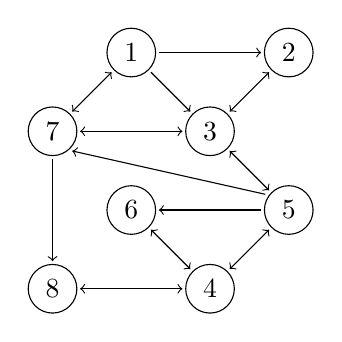
\begin{tikzpicture}
            \draw (0,0) node[circle,draw]{3};
            \draw (-1,1) node[circle,draw]{1};
            \draw (1,1) node[circle,draw]{2};
            \draw (-1,-1) node[circle,draw]{6};
            \draw (1,-1) node[circle,draw]{5};
            \draw (0,-2) node[circle,draw]{4};
            \draw (-2,0) node[circle,draw]{7};
            \draw (-2,-2) node[circle,draw]{8};
        %
            \draw[<-] (-0.25,0.25) -- (-0.75,0.75);
            \draw[->] (-0.65,1) -- (0.65,1);
            \draw[<->] (0.25,0.25) -- (0.75,0.75);
            \draw[<->] (0.25,-0.25) -- (0.75,-0.75);
            \draw[->] (0.65,-1) -- (-0.65,-1);
            \draw[<->] (-0.75,-1.25) -- (-.25,-1.75);
            \draw[<->] (0.75,-1.25) -- (0.25,-1.75);
            \draw[<->] (-1.75,0.25) -- (-1.25,0.75);
            \draw[<->] (-1.65,0) -- (-0.35,0);
            \draw[<-] (-1.75,-0.25) -- (0.7,-0.8);
            \draw[->] (-2,-0.35) -- (-2,-1.65);
            \draw[<->] (-1.65,-2) -- (-0.35,-2);
        \end{tikzpicture}
    \end{center}
    \caption{Graph of a web with eight pages.}
    \label{fig:graph2}
\end{figure}


\begin{problem}
    One thing that we didn't consider in this version of the Google Page Rank algorithm is
    the random behavior of humans.  One, admittedly slightly naive, modification that we
    can make to the present algorithm is to assume that the person surfing the web will
    randomly jump to any other page in the web at any time.  For example, if someone is on
    page 1 in Figure \ref{fig:graph2} then they could randomly jump to any page 2 - 8.
    They also have links to pages 2, 3, and 7.  That is a total of 10 possible next steps
    for the web surfer.  There is a $2/10$ chance of heading to page 2.  One of those is
    following the link from page 1 to page 2 and the other is a random jump to page 2
    without following the link.  Similarly, there is a $2/10$ chance of
    heading to page 3, $2/10$ chance of heading to page 7, and a $1/10$ chance of randomly
    heading to any other page.

    Implement this new algorithm, called the {\it random surfer algorithm}, on the web in
    Figure \ref{fig:graph2}.  Compare your ranking to the non-random surfer results from
    the previous problem.
\end{problem}



\newpage\section{Principal Component Analysis (Incomplete)}

\newpage\section{Building PDE's From Conservation Laws}

In this section
we'll give a more analytic introduction to most of the primary partial
differential equations of interest in basic mathematical physics.  We will make reference
to Fick's Law for mass transport and Fourier's Law for thermal transport, so interested
readers should dig deeper by examining the relevant Wikipedia pages or other sources.
  
Conservation laws pervade all of physics -- conservation of energy, conservation of
momentum, and conservation of mass.  These laws are sometimes stated colloquially as
{\it energy (or momentum or mass) can neither be created nor destroyed}, but this phrase
is not super helpful mathematically.  We start this section with a brief mathematical
derivation of a {\it general conservation law} to further clarify what we mean
mathematically.  The resulting general conservation law will be a
partial differential equation that can be used to mathematically express the physical laws
of conservation of mass, momentum, or
energy.

Let $u$ be the quantity you are trying to conserve, $\bq$ be the flux of that quantity,
and $f$ be any source of that quantity.  For example, if we are to derive a conservation
of energy equation, $u$ might be energy, $\bq$ might be temperature flux, and $f$ might be
a temperature source (or sink).

\subsection*{Derivation of General Balance Law}
Let $\Omega$ be a fixed volume and denote the boundary of this volume by $\partial
\Omega$. The rate at which $u$ is changing in time throughout $\Omega$ needs to be
balanced by the rate at which $u$ leaves the volume plus any sources of $u$.
Mathematically, this means that
\begin{flalign}
    \pd{ }{t} \iiint_{\Omega} u dV = -\iint_{\partial \Omega} \bq \cdot n dA +
    \iiint_\Omega f dV.
    \label{eqn:global_balance}
\end{flalign}
This is a global balance law in the sense that it holds for all volumes $\Omega$.  The
mathematical 
troubles here are two fold: (1) there are many integrals, and (2) there are really two variables
($u$ and $q$ since $f=f(u,x,t)$) so the equation is not closed.  In order to mitigate
that fact we apply the divergence theorem to the first term on the right-hand side of
\eqref{eqn:global_balance} to get
\begin{flalign}
    \pd{ }{t} \iiint_{\Omega} u dV = -\iiint_{\Omega} \nabla \cdot \bq dV +
    \iiint_\Omega f dV.
    \label{eqn:global_balance2}
\end{flalign}

Gathering all of the terms on the right of \eqref{eqn:global_balance2}, interchanging the integral and the derivative on
the left (since the volume is not changing in time), and rewriting gives
\begin{flalign}
    \iiint_\Omega \left( \pd{u}{t} + \nabla \cdot \bq \right) dV = \iiint_\Omega f dV
    \label{eqn:global_balance3}
\end{flalign}
If we presume that this equation holds for all volumes $\Omega$ then the integrands must
be equal and we get the local balance law
\begin{flalign}
    \pd{u}{t} + \nabla \cdot \bq = f.
    \label{eqn:local_balance}
\end{flalign}

Equation \eqref{eqn:local_balance} is an expression of the balances of changes in time to
changes in space of a conserved quantity such as mass, momentum, or energy.  What remains
is to make clear the meaning and functional form of the flux $\bq$ and the source function
$f$.

\subsection*{Simplification of the Local Balance Law}
In equation \eqref{eqn:local_balance} it is often assumed that the system is free of
external sources.  In this case we set $f$ to zero and obtain the source-free balance law
\begin{flalign}
    \pd{u}{t} + \nabla \cdot \bq = 0.
    \label{eqn:local_source_free}
\end{flalign}
It is this form of balance law where many of the most interesting and important partial
differential equations come from.  In particular consider the following two cases: mass
balance and energy balance.
\subsection*{Mass Balance}
In mass balance we take $u$ to either be the density of a substance (e.g. in the case of
liquids) or the concentration of a substance in a mixture (e.g. in the case of
gasses). If $C$ is the mass concentration of a substance in a gas then the flux of that
substance is given via Fick's Law as
\begin{flalign}
    \bq = -k \nabla C.
    \label{eqn:fick}
\end{flalign}
Combining \eqref{eqn:fick} with \eqref{eqn:local_source_free} (and assuming that $k$ is
independent of space, time, and concentration) gives
\begin{flalign}
    \pd{C}{t} = k \nabla \cdot \nabla C. 
    \label{eqn:fick2_simp}
\end{flalign}
In the presence of external sources of mass, \eqref{eqn:fick2_simp} is
\begin{flalign}
    \pd{C}{t} = k \nabla \cdot \nabla C + f(x).
    \label{eqn:fick3}
\end{flalign}
Expanding the Laplacian operator on the right-hand side of \eqref{eqn:fick3} we get
\begin{flalign}
    \pd{C}{t} = k\left( \pdd{C}{x} + \pdd{C}{y} + \pdd{C}{z} \right) + f(x)
    \label{eqn:fick3_expanded}
\end{flalign}
where the reader should note that this can be easily simplified in 1 or 2 spatial
dimensions.
% \begin{problem}
%     What does \eqref{eqn:fick3} equation look like in terms of spatial derivatives on the
%     right-hand side?
%     \begin{flalign*}
%         \pd{C}{t} &= \underline{\hspace{2in}} \quad \text{(1 Spatial Dimension)} \\
%         \pd{C}{t} &= \underline{\hspace{2in}} \quad \text{(2 Spatial Dimensions)} \\
%         \pd{C}{t} &= \underline{\hspace{2in}} \quad \text{(3 Spatial Dimensions)}
%     \end{flalign*}
% \end{problem}

\subsection*{Energy Balance}
The energy balance equation is essentially the same as the mass balance equation.  If $u$
is temperature then the flux of temperature is given by Fourier's Law for heat conduction
\begin{flalign}
    \bq = -k\nabla T.
    \label{eqn:fourier}
\end{flalign}
Making the same simplifications as in the mass balance equation we arrive at
\begin{flalign}
    \pd{T}{t} = k \nabla \cdot \nabla T.
    \label{eqn:fourier2}
\end{flalign}
In the presence of external sources of heat, \eqref{eqn:fourier2} becomes
\begin{flalign}
    \pd{T}{t} = k \nabla \cdot \nabla T + f(x).
    \label{eqn:fourier3}
\end{flalign}
Expanding the Laplacian operator on the right-hand side of \eqref{eqn:fourier3} we get
\begin{flalign}
    \pd{T}{t} = k\left( \pdd{T}{x} + \pdd{T}{y} + \pdd{T}{z} \right) + f(x)
    \label{eqn:fourier3_expanded}
\end{flalign}
where the reader should note that this can be easily simplified in 1 or 2 spatial
dimensions.
% \begin{problem}
%     What does \eqref{eqn:fourier3} equation look like in terms of spatial derivatives on the
%     right-hand side?
%     \begin{flalign*}
%         \pd{T}{t} &= \underline{\hspace{2in}} \quad \text{(1 Spatial Dimension)} \\
%         \pd{T}{t} &= \underline{\hspace{2in}} \quad \text{(2 Spatial Dimensions)}\\
%         \pd{T}{t} &= \underline{\hspace{2in}} \quad \text{(3 Spatial Dimensions)}
%     \end{flalign*}
% \end{problem}



\subsection*{Laplace's Equation and Poisson's Equation}
Equations \eqref{eqn:fick3} and \eqref{eqn:fourier3} are the same partial differential
equation for two very important physical phenomenon; mass and heat transfer.  In the case
where time is allowed to run to infinity and no external sources of mass or energy are
included these equations reach a steady state solution (no longer changing in time) and we
arrive at Laplace's Equation
\begin{flalign}
    \nabla \cdot \nabla u = 0.
    \label{eqn:laplace}
\end{flalign}
Laplace's equation is actually a statement of minimal energy as well as steady state heat
or temperature.  We can see this since entropy always drives systems from high energy to
low energy, and if we have reached a steady state then we must have also reached a surface
of minimal energy.

Equation \eqref{eqn:laplace} is sometimes denoted as $\nabla \cdot \nabla u = \nabla^2 u =
\Delta u$, and in terms of the partial derivatives it is written as
\begin{flalign*}
    \pdd{u}{x} + \pdd{u}{y} + \pdd{u}{z} = 0.
% V    0 &= \underline{\hspace{2in}} \quad \text{(1 Spatial Dimension)} \\
%     0 &= \underline{\hspace{2in}} \quad \text{(2 Spatial Dimensions)} \\
%     0 &= \underline{\hspace{2in}} \quad \text{(3 Spatial Dimensions)} 
\end{flalign*}

If there is a time-independent external source the right-hand side of
\eqref{eqn:laplace} will be non-zero and we arrive at Poisson's equation:
\begin{flalign}
    \nabla \cdot \nabla u = -f(x).
    \label{eqn:poisson}
\end{flalign}
Note that the negative on the right-hand side comes from the fact that
$\pd{u}{t} = k \nabla \cdot \nabla u + f(x)$ and $\pd{u}{t} \to 0$.  Technically we are
absorbing the constant $k$ into $f$ (that is ``$f$'' is really ``$f/k$'').  Also
note that in many instances the value of $k$ is not constant and cannot therefore be pulled
out of the derivative without a use of the product rule.

Let's summarize:
\begin{center}
    \begin{tabular}{|c|c|c|}
        \hline
        Name of PDE & PDE & What the PDE Models \\ \hline \hline
        The Heat Equation & $\ds \pd{u}{t} = k \nabla \cdot \nabla u + f(x)$ & Diffusion \\
        Laplace's Equation & $\ds k \nabla \cdot \nabla u =-f(x)$ & Minimal Energy
        Surfaces \\
%         The Wave Equation & $\ds \pdd{u}{t} = k \nabla \cdot \nabla u + f(x)$ & Wave
%         phenomena \\
        \hline
    \end{tabular}
\end{center}

Further discussion of the origins of the wave equation and other interesting PDE's is left
to the reader.

